\documentclass[lettersize,journal]{IEEEtran}
\usepackage{amsmath,amsfonts}
\usepackage{tikz}
\usepgflibrary{plotmarks}
\usepackage{amssymb}
\usepackage{amsmath}

\begin{document}

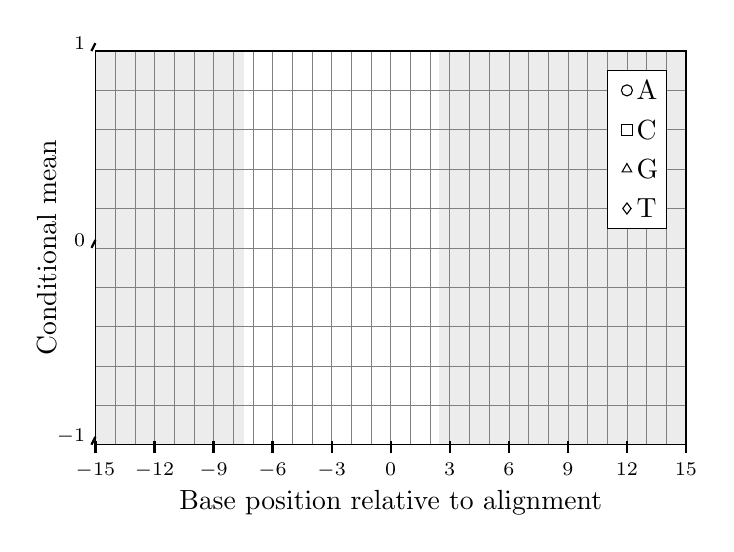
\begin{tikzpicture} [x=0.25cm,y=2.5cm]

\draw[help lines, ystep=0.2, xstep=1] (-15,-1) grid (15,1);
\draw[fill, color=gray, opacity=0.15] (-15,-1) rectangle (-7.5,1);
\draw[fill, color=gray, opacity=0.15] (2.5,-1) rectangle (15,1);
\draw (-15,-1) rectangle (15,1);
\foreach \x in {-15,-12,...,15} {
	\draw[thick] (\x,-1)+(0,0.5mm) -- +(0,-1.0mm) node [anchor=north] {\scriptsize $\x$};
}
\foreach \y in {-1,0,...,1} {
	\draw[thick] (-15,\y)+(-0.5mm,0) -- +(0,1.0mm) node [anchor=east] {\scriptsize $\y$};
}
\draw[mark=o] plot file{figure/ConditionalSignalValueA.txt};
\draw[mark=square] plot file{figure/ConditionalSignalValueC.txt};
\draw[mark=triangle] plot file{figure/ConditionalSignalValueG.txt};
\draw[mark=diamond] plot file{figure/ConditionalSignalValueT.txt};

\draw[fill, color=white] (11,0.1) rectangle (14,0.9);
\draw[] (11,0.1) rectangle (14,0.9);
\draw plot[only marks,mark=o] coordinates{(12,0.8)} node [right] {A};
\draw plot[only marks,mark=square] coordinates{(12,0.6)} node [right] {C};
\draw plot[only marks,mark=triangle] coordinates{(12,0.4)} node [right] {G};
\draw plot[only marks,mark=diamond] coordinates{(12,0.2)} node [right] {T};

\node at (0,-1.18) [anchor=north] {Base position relative to alignment};
\node at (-16.5,0) [anchor=south, rotate=90] {Conditional mean};

\end{tikzpicture}

\end{document}